
\begin{center}
    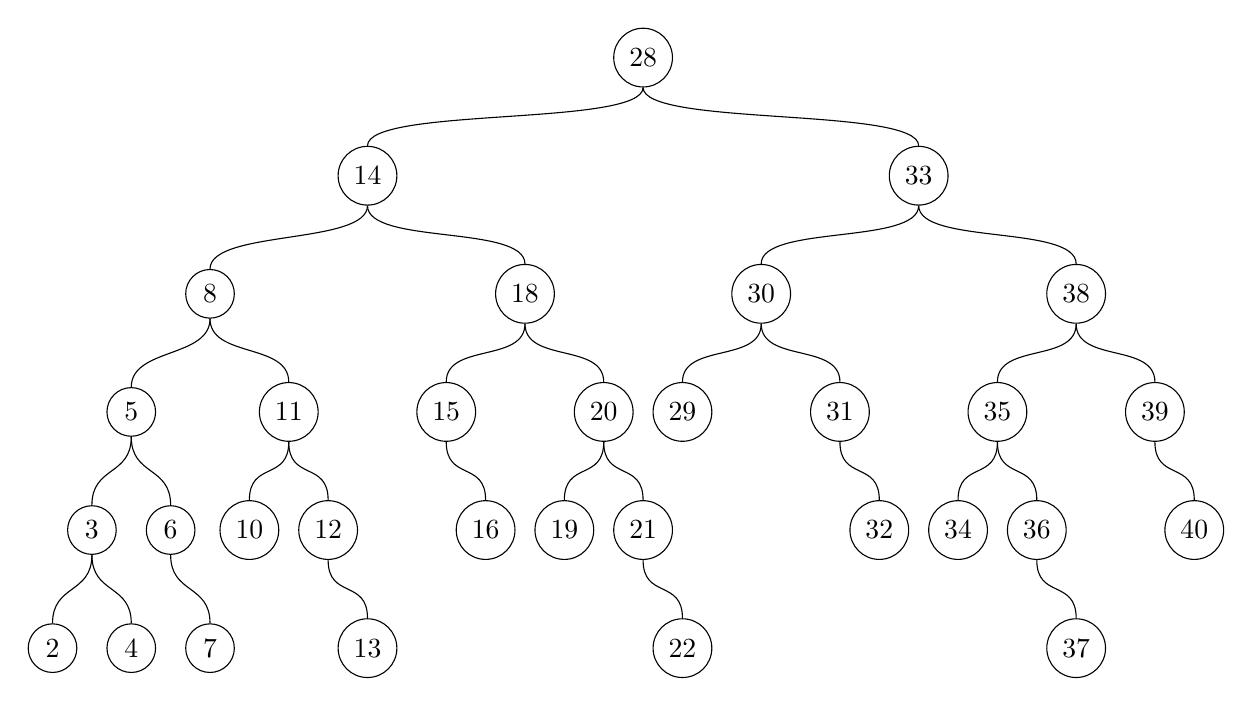
\begin{tikzpicture}[
       edge from parent path=
    {(\tikzparentnode.south) .. controls +(0,-.5) and +(0,.5)
                             .. (\tikzchildnode.north)},
    level 1/.style={sibling distance=7cm},                        
    level 2/.style={sibling distance=4cm},                         
    level 3/.style={sibling distance=2cm},
    level 4/.style={sibling distance=1cm},
   every node/.style={draw,circle},
   label distance=-1mm]
   
\node {28}
    child {node {14}
        child {node {8}
            child {node {5}
                child {node {3}
                    child {node {2}}
                    child {node {4}}
                }
                child {node {6}
                    child[missing] {}
                    child {node {7}}
                }
            }
            child {node {11}
                child {node {10}}
                child {node {12}
                    child[missing] {}   
                    child {node {13}}
                }
            }
        }
        child {node {18}
            child {node {15}
                child[missing] {}   
                child {node {16}}
            }
            child {node {20}
                child {node {19}}
                child {node {21}
                    child[missing] {}   
                    child {node {22}}
                }
            }
        }
    }   
    child {node {33}
        child {node {30}
            child {node {29}}
            child {node {31}
                    child[missing] {}
                    child {node {32}}
                }
            }
        child {node {38}
            child {node {35}
                child {node {34}}
                child {node {36}
                    child[missing] {}
                    child {node {37}}
                }
            }
            child {node {39}
                child[missing] {}
                child {node {40}}
            }
        }
    };

\end{tikzpicture}
\end{center}